\documentclass{article}\usepackage[]{graphicx}\usepackage[]{xcolor}
% maxwidth is the original width if it is less than linewidth
% otherwise use linewidth (to make sure the graphics do not exceed the margin)
\makeatletter
\def\maxwidth{ %
  \ifdim\Gin@nat@width>\linewidth
    \linewidth
  \else
    \Gin@nat@width
  \fi
}
\makeatother

\definecolor{fgcolor}{rgb}{0.345, 0.345, 0.345}
\newcommand{\hlnum}[1]{\textcolor[rgb]{0.686,0.059,0.569}{#1}}%
\newcommand{\hlsng}[1]{\textcolor[rgb]{0.192,0.494,0.8}{#1}}%
\newcommand{\hlcom}[1]{\textcolor[rgb]{0.678,0.584,0.686}{\textit{#1}}}%
\newcommand{\hlopt}[1]{\textcolor[rgb]{0,0,0}{#1}}%
\newcommand{\hldef}[1]{\textcolor[rgb]{0.345,0.345,0.345}{#1}}%
\newcommand{\hlkwa}[1]{\textcolor[rgb]{0.161,0.373,0.58}{\textbf{#1}}}%
\newcommand{\hlkwb}[1]{\textcolor[rgb]{0.69,0.353,0.396}{#1}}%
\newcommand{\hlkwc}[1]{\textcolor[rgb]{0.333,0.667,0.333}{#1}}%
\newcommand{\hlkwd}[1]{\textcolor[rgb]{0.737,0.353,0.396}{\textbf{#1}}}%
\let\hlipl\hlkwb

\usepackage{framed}
\makeatletter
\newenvironment{kframe}{%
 \def\at@end@of@kframe{}%
 \ifinner\ifhmode%
  \def\at@end@of@kframe{\end{minipage}}%
  \begin{minipage}{\columnwidth}%
 \fi\fi%
 \def\FrameCommand##1{\hskip\@totalleftmargin \hskip-\fboxsep
 \colorbox{shadecolor}{##1}\hskip-\fboxsep
     % There is no \\@totalrightmargin, so:
     \hskip-\linewidth \hskip-\@totalleftmargin \hskip\columnwidth}%
 \MakeFramed {\advance\hsize-\width
   \@totalleftmargin\z@ \linewidth\hsize
   \@setminipage}}%
 {\par\unskip\endMakeFramed%
 \at@end@of@kframe}
\makeatother

\definecolor{shadecolor}{rgb}{.97, .97, .97}
\definecolor{messagecolor}{rgb}{0, 0, 0}
\definecolor{warningcolor}{rgb}{1, 0, 1}
\definecolor{errorcolor}{rgb}{1, 0, 0}
\newenvironment{knitrout}{}{} % an empty environment to be redefined in TeX

\usepackage{alltt}
\usepackage[margin=1.0in]{geometry} % To set margins
\usepackage{amsmath}  % This allows me to use the align functionality.
                      % If you find yourself trying to replicate
                      % something you found online, ensure you're
                      % loading the necessary packages!
\usepackage{amsfonts} % Math font
\usepackage{fancyvrb}
\usepackage{hyperref} % For including hyperlinks
\usepackage[shortlabels]{enumitem}% For enumerated lists with labels specified
                                  % We had to run tlmgr_install("enumitem") in R
\usepackage{float}    % For telling R where to put a table/figure
\usepackage{natbib}        %For the bibliography
\bibliographystyle{apalike}%For the bibliography
\IfFileExists{upquote.sty}{\usepackage{upquote}}{}
\begin{document}

In lecture 16, we looked at precipitation amounts in Madison County (at 
Morrisville station). We found that the Weibull distribution had a good fit
to the monthly precipitation amounts.\\

We found that the MLEs for the Weibull distribution were 
\begin{align*}
    \hat{a}&=2.1871\\
    \hat{\sigma}&=3.9683
\end{align*}
and
\[-\mathcal{L}(\{\hat{a}, \hat{\sigma}\}|\mathbf{x}) = 2166.496\]
is the realized negative log-likelihood.
Note this means that the log-likelihood is
\[\mathcal{L}(\{\hat{a}, \hat{\sigma}\}|\mathbf{x}) = -2166.496,\]
and the usual likelihood is
\[L(\{\hat{a}, \hat{\sigma}\}|\mathbf{x}) = e^{\left[\mathcal{L}(\{\hat{a}, \hat{\sigma}\}|\mathbf{x})\right]} \approx e^{-2166.496}\]
which \texttt{R} cannot differentiate from 0.

\begin{enumerate}
  \item Someone asked ``why Weibull?" in class. That is, why wouldn't we use 
  another right-skewed distribution like the Gamma (see Lecture 15), or
  the Log-Normal (see Lecture 17).
  \begin{enumerate}
    \item Compute the MLEs for these data using a Gamma distribution.
\begin{knitrout}\scriptsize
\definecolor{shadecolor}{rgb}{0.969, 0.969, 0.969}\color{fgcolor}\begin{kframe}
\begin{alltt}
\hldef{data.precip} \hlkwb{=} \hlkwd{read_csv}\hldef{(}\hlsng{"data.csv"}\hldef{)}

\hldef{mlegamma} \hlkwb{<-} \hlkwa{function}\hldef{(}\hlkwc{data}\hldef{,} \hlkwc{par}\hldef{,} \hlkwc{neg}\hldef{=F)\{}
  \hldef{alpha} \hlkwb{<-} \hldef{par[}\hlnum{1}\hldef{]}
  \hldef{beta} \hlkwb{<-} \hldef{par[}\hlnum{2}\hldef{]}

  \hldef{loglik} \hlkwb{<-} \hlkwd{sum}\hldef{(}\hlkwd{log}\hldef{(}\hlkwd{dgamma}\hldef{(}\hlkwc{x}\hldef{=data,} \hlkwc{shape}\hldef{=alpha,} \hlkwc{rate}\hldef{=beta)))}

  \hlkwd{return}\hldef{(}\hlkwd{ifelse}\hldef{(neg,} \hlopt{-}\hldef{loglik, loglik))}
\hldef{\}}

\hldef{mles} \hlkwb{<-} \hlkwd{optim}\hldef{(}\hlkwc{par} \hldef{=} \hlkwd{c}\hldef{(}\hlnum{1}\hldef{,}\hlnum{1}\hldef{),}
           \hlkwc{fn} \hldef{= mlegamma,}
           \hlkwc{data}\hldef{=data.precip}\hlopt{$}\hldef{Precipitation,}
           \hlkwc{neg}\hldef{=T)}
\hldef{(alpha.hat.mle} \hlkwb{<-} \hldef{mles}\hlopt{$}\hldef{par[}\hlnum{1}\hldef{])}
\end{alltt}
\begin{verbatim}
## [1] 4.174581
\end{verbatim}
\begin{alltt}
\hldef{(beta.hat.mle} \hlkwb{<-} \hldef{mles}\hlopt{$}\hldef{par[}\hlnum{2}\hldef{])}
\end{alltt}
\begin{verbatim}
## [1] 1.189099
\end{verbatim}
\begin{alltt}
\hlcom{#LOG LIKELIHOOD }
\hldef{(}\hlkwd{sum}\hldef{(}\hlkwd{log}\hldef{(}\hlkwd{dgamma}\hldef{(}\hlkwc{x}\hldef{=data.precip}\hlopt{$}\hldef{Precipitation,} \hlkwc{shape} \hldef{= alpha.hat.mle,} \hlkwc{rate} \hldef{= beta.hat.mle))))}
\end{alltt}
\begin{verbatim}
## [1] -2151.149
\end{verbatim}
\end{kframe}
\end{knitrout}

    \begin{align*}
    \hat{\alpha}&=4.1746\\
    \hat{\beta}&=1.1891
\end{align*}
    \item Compute the MLEs for these data using the Log-Normal distribution.
\begin{knitrout}\scriptsize
\definecolor{shadecolor}{rgb}{0.969, 0.969, 0.969}\color{fgcolor}\begin{kframe}
\begin{alltt}
\hldef{data.precip} \hlkwb{=} \hlkwd{read_csv}\hldef{(}\hlsng{"data.csv"}\hldef{)}

\hldef{mlelognormal} \hlkwb{<-} \hlkwa{function}\hldef{(}\hlkwc{data}\hldef{,} \hlkwc{par}\hldef{,} \hlkwc{neg}\hldef{=F)\{}
  \hldef{meanlog} \hlkwb{<-} \hldef{par[}\hlnum{1}\hldef{]}
  \hldef{sdlog} \hlkwb{<-} \hldef{par[}\hlnum{2}\hldef{]}

  \hldef{loglik} \hlkwb{<-} \hlkwd{sum}\hldef{(}\hlkwd{log}\hldef{(}\hlkwd{dlnorm}\hldef{(}\hlkwc{x}\hldef{=data,} \hlkwc{meanlog}\hldef{=meanlog,} \hlkwc{sdlog}\hldef{=sdlog)))}

  \hlkwd{return}\hldef{(}\hlkwd{ifelse}\hldef{(neg,} \hlopt{-}\hldef{loglik, loglik))}
\hldef{\}}

\hldef{mles} \hlkwb{<-} \hlkwd{optim}\hldef{(}\hlkwc{par} \hldef{=} \hlkwd{c}\hldef{(}\hlnum{1}\hldef{,}\hlnum{1}\hldef{),}
          \hlkwc{fn} \hldef{= mlelognormal,}
          \hlkwc{data}\hldef{=data.precip}\hlopt{$}\hldef{Precipitation,}
          \hlkwc{neg}\hldef{=T)}
\hldef{(meanlog} \hlkwb{<-} \hldef{mles}\hlopt{$}\hldef{par[}\hlnum{1}\hldef{])}
\end{alltt}
\begin{verbatim}
## [1] 1.131261
\end{verbatim}
\begin{alltt}
\hldef{(sdlog} \hlkwb{<-} \hldef{mles}\hlopt{$}\hldef{par[}\hlnum{2}\hldef{])}
\end{alltt}
\begin{verbatim}
## [1] 0.5333417
\end{verbatim}
\begin{alltt}
\hlcom{#LOG LIKELIHOOD}
\hldef{(}\hlkwd{sum}\hldef{(}\hlkwd{log}\hldef{(}\hlkwd{dlnorm}\hldef{(}\hlkwc{x}\hldef{=data.precip}\hlopt{$}\hldef{Precipitation,} \hlkwc{meanlog}\hldef{=meanlog,} \hlkwc{sdlog}\hldef{=sdlog))))}
\end{alltt}
\begin{verbatim}
## [1] -2204.201
\end{verbatim}
\end{kframe}
\end{knitrout}
    \begin{align*}
    \hat{\mu}&=1.1312\\
    \hat{\sigma}&=0.5333
\end{align*}
    \item Compute the likelihood ratio to compare the Weibull and the Gamma distribution. 
    Which has a better fit according to the likelhiood ratio?
    \[Q = \frac{L(\{\hat{a}, \hat{\sigma}\}|\mathbf{x})}{L(\{\hat{\alpha}, \hat{\beta}\}|\mathbf{x})}=e^{\left[\mathcal{L}(\{\hat{a}, \hat{\sigma}\}|\mathbf{x}) - \mathcal{L}(\{\hat{\alpha}, \hat{\beta}\}|\mathbf{x})\right]} \approx e^{-15.34738}\]
    \textbf{Explanation:} Since the Q-value is less than one then we know that the Gamma distribution has a better fit according to the ratio. \\
    \item Compute the likelihood ratio to compare the Weibull and the Log-Normal distribution.
    Which has a better fit according to the likelihood ratio?
    \[Q = \frac{L(\{\hat{a}, \hat{\sigma}\}|\mathbf{x})}{L(\{\hat{\mu}, \hat{\sigma}\}|\mathbf{x})}=e^{\left[\mathcal{L}(\{\hat{a}, \hat{\sigma}\}|\mathbf{x}) - \mathcal{L}(\{\hat{\mu}, \hat{\sigma}\}|\mathbf{x})\right]} \approx e^{37.70453}\]
    \textbf{Explanation:} Since the Q-value is greater than one then we know that the Weibull distribution has a better fit according to the ratio. \\
    \item Compute the likelihood ratio to compare the Gamma and the Log-Normal distribution.
    Which has a better fit according to the likelhiood ratio?
    \[Q = \frac{L(\{\hat{\alpha}, \hat{\beta}\}|\mathbf{x})}{L(\{\hat{\mu}, \hat{\sigma}\}|\mathbf{x})}=e^{\left[\mathcal{L}(\{\hat{\alpha}, \hat{\beta}\}|\mathbf{x}) - \mathcal{L}(\{\hat{\mu}, \hat{\sigma}\}|\mathbf{x})\right]} \approx e^{53.05191}\]
    \textbf{Explanation:} Since the Q-value is greater than one then we know that the Gamma distribution has a better fit according to the ratio. \\
  \end{enumerate}
  \item Optional Coding Challenge. Choose the ``best" distribution and refit the
  model by season.
  \begin{enumerate}
    \item Fit the Distribution for Winter (December-February).
    \item Fit the Distribution for Spring (March-May).
    \item Fit the Distribution for Summer (June-August).
    \item Fit the Distribution for Fall (September-November).
    \item Plot the four distributions in one plot using \texttt{cyan3} for Winter,
    \texttt{chartreuse3} for Spring, \texttt{red3} for Summer, and \texttt{chocolate3}
    for Fall. Note any similarities/differences you observe across the seasons.
    \begin{figure}[H]
    \begin{center}
\begin{knitrout}
\definecolor{shadecolor}{rgb}{0.969, 0.969, 0.969}\color{fgcolor}
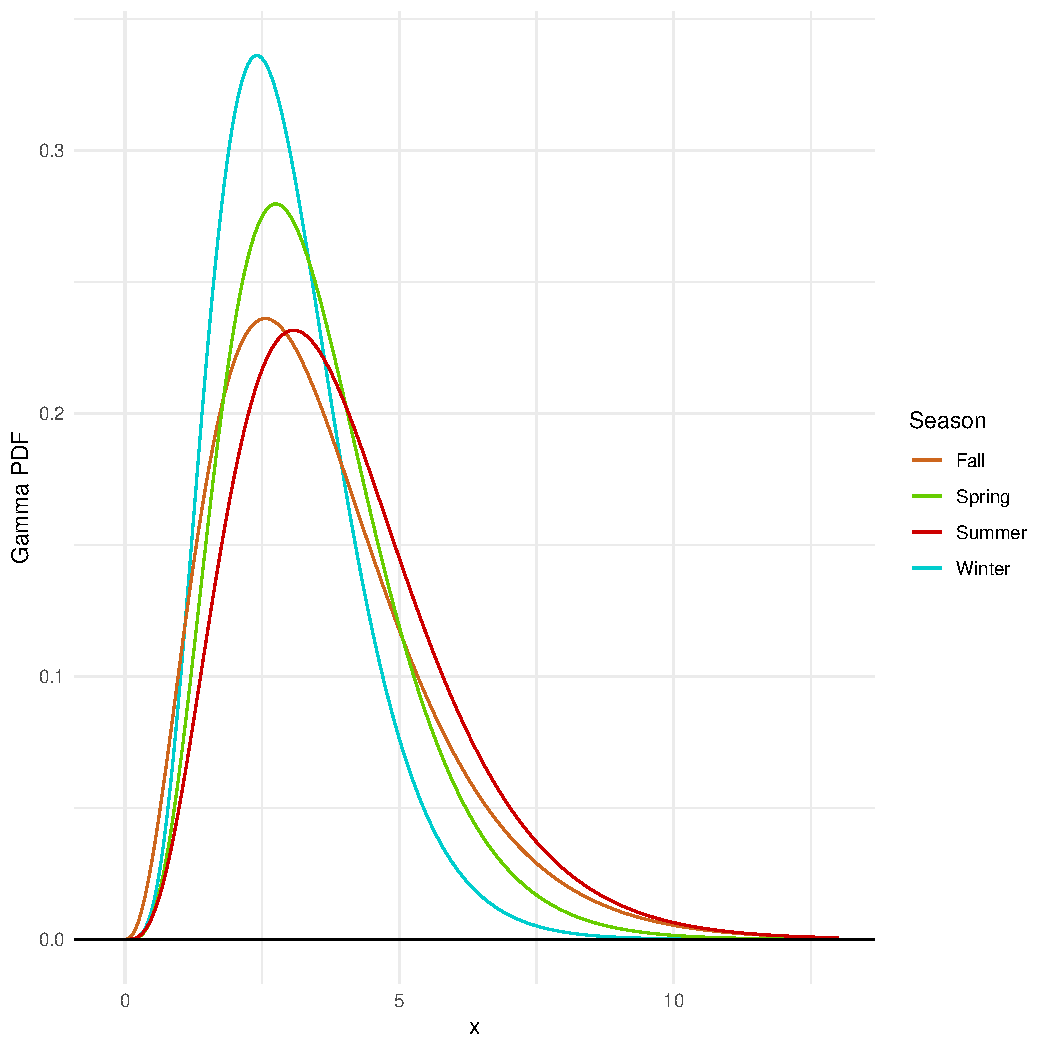
\includegraphics[width=\maxwidth]{figure/unnamed-chunk-4-1} 
\end{knitrout}
\caption{Gamma Dist. for Each Season}
\label{Figure 1}
\end{center}
\end{figure}
  \end{enumerate}
\end{enumerate}

\bibliography{bibliography}
\end{document}
